%==============================================================================%
%========================|     CHAPTER 2 Literature    |=======================%
%==============================================================================%
\chapter{Literature Review} \label{chap:Literature}
This chapter reviews the literature on Breach and Attack Simulation (BAS) and its role in proactive defense testing. It commences with the core concepts before analyzing the design and capabilities of MITRE Caldera, Infection Monkey, and Atomic Red Team. To conclude, the chapter discusses earlier comparative studies that guided the framework of this research.

%-----------------------------|    2.1 Overview_BAS    |-----------------------------------|
\section{Overview of Breach and Attack Simulation (BAS)}\label{sec:Overview_BAS}
Breach and Attack Simulation (BAS) is a critical component of modern cybersecurity defense strategies. It is a proactive and automated methodology for continuously testing an organization's security posture by safely emulating real-world cyberattacks in a controlled environment\cite{picus_bas}. Unlike traditional security tools that rely on heuristic analysis, BAS provides empirical evidence of defense effectiveness by directly measuring the performance of security controls against simulated threats. This helps to uncover critical blind spots, misconfigurations, and silent failures that are often missed by conventional assessments like vulnerability scanning or penetration testing\cite{mindgard_redteam}.

An effective BAS platform is built upon several core components that collectively enable a robust and continuous validation process. At its foundation is the attack simulation engine, which emulates real-world cyberattacks using a library of known tactics, techniques, and procedures (TTPs). This engine is supported by a rich scenario library and playbooks that contain predefined attack scenarios, mimicking the behaviors of different threat actors and malware families. The platform's primary function is security control validation, assessing the effectiveness of existing defenses such as firewalls, Endpoint Detection and Response (EDR), and Security Information and Event Management (SIEM) systems.

For maximum efficiency, BAS solutions feature automated and continuous testing, allowing for scheduled attack simulations to ensure security defenses remain effective over time. During and after a simulation, data collection and analytics capture detailed logs and insights, providing the necessary information to identify gaps and areas for improvement. The ultimate value of a BAS platform is derived from its ability to conduct risk and impact assessments, which evaluate the potential business impact of identified vulnerabilities and prioritize remediation efforts. Finally, the platform generates comprehensive reporting and remediation guidance, offering actionable insights to security teams to help them efficiently strengthen their security posture.

%-------------------------|    2.2 Opensource_BAS    |-------------------------------------|
\section{Open-Source Breach Attack Simulation Tools}\label{sec:Opensource_BAS}
As the demand for continuous security validation grows, open-source Breach and Attack Simulation (BAS) tools have gained significant traction among organizations seeking cost-effective alternatives to commercial platforms\cite{yuceel2025}. These tools offer practical means to emulate cyberattacks, assess security controls, and identify vulnerabilities without the financial burden associated with enterprise-grade solutions.

Open-source BAS tools vary in scope, complexity, and focus. Some are designed for red team operations and adversary emulation, while others prioritize endpoint testing or network resilience. Despite their differences, these tools share a common goal: to provide actionable insights into an organization’s security posture through realistic and repeatable attack simulations.

\textbf{Prominent open-source BAS tools include:}
\begin{itemize}
    \item \textbf{MITRE Caldera:} A modular platform developed by MITRE that automates adversary emulation using the MITRE ATT\&CK framework. It supports custom agents, flexible operation chains, and integration with other security tools\cite{caldera_docs}.
    \item \textbf{Infection Monkey:} Developed by Guardicore (now part of Akamai), this tool simulates lateral movement and network-based attacks to evaluate internal network resilience. It provides detailed reports on misconfigurations and vulnerabilities\cite{monkey_docs}.
    \item \textbf{Atomic Red Team:} Maintained by Red Canary, this framework offers a library of small, discrete tests mapped to ATT\&CK techniques. It is lightweight, highly customizable, and ideal for validating specific security controls\cite{atomic_docs}.
\end{itemize}

These tools are increasingly adopted by security teams, researchers, and educators due to their accessibility, transparency, and community support. While they may lack some of the advanced features found in commercial BAS platforms—such as centralized dashboards, enterprise integrations, or automated remediation—they offer a valuable starting point for organizations aiming to strengthen their cybersecurity posture through hands-on testing\cite{redcanary_compare}.

%-------------------------|    2.3 MITRE Caldera    |------------------------------|
\section{MITRE Caldera}\label{sec:Caldera}
MITRE Caldera\cite{caldera_docs} is an open-source adversary emulation platform developed by The MITRE Corporation to enhance cybersecurity defenses by automating the execution of realistic cyber-attack and defense scenarios, referred to as operations. The framework's core purpose is to validate security controls, train blue teams, and evaluate an organization's security posture against known adversarial Tactics, Techniques, and Procedures (TTPs).

Caldera is architected as a modular, knowledge-driven system, utilizing key components like Agents (the executable implant, typically Sandcat) that communicate with the C2 server, and Abilities, which are modular implementations of single ATT\&CK techniques. These abilities are grouped into Adversary Profiles and executed during an operation, with the order determined by specialized Planners (e.g., atomic or batch).

The Caldera interface adapts its available toolset based on the operator's role, as observed in the sidebar configuration. The \textbf{Red Dashboard} (Figure~\ref{fig:Caldera_dashboard_red}) exposes the full suite of offensive plugins, including `access`, `atomic`, and `manx`, enabling operators to launch and manage attacks. In contrast, the \textbf{Blue Dashboard} (Figure~\ref{fig:Caldera_dashboard_blue}) streamlines the interface for defensive operations; it removes the offensive toolsets and introduces the `response` plugin, which facilitates autonomous defensive actions. While the central metrics remain consistent, the sidebar functionality is distinct for each role.

\begin{figure}
    \centering
    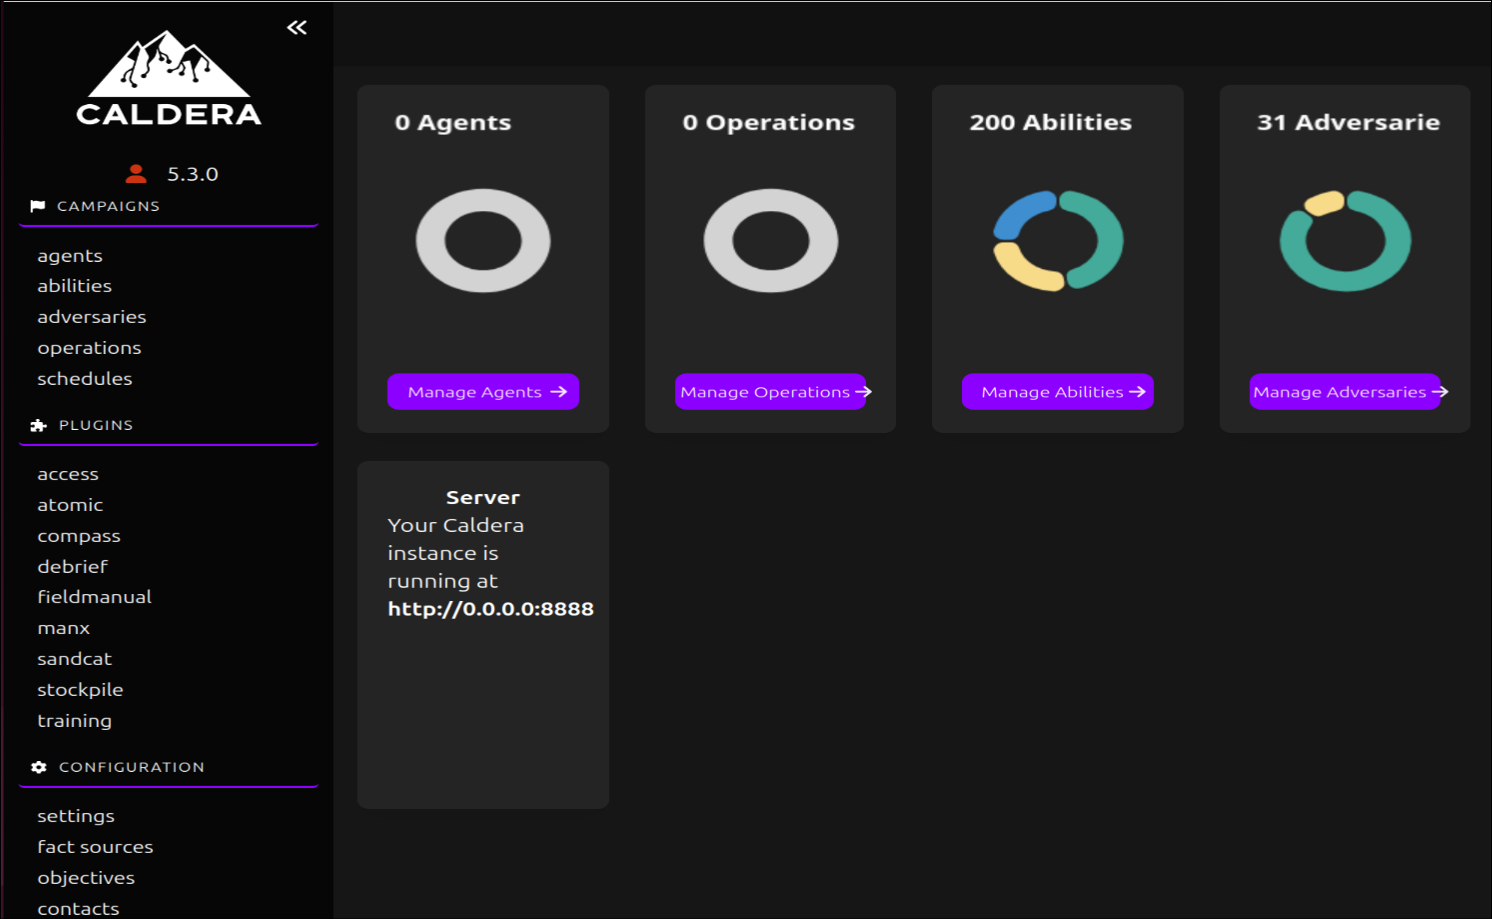
\includegraphics[width=1\linewidth]{figures/Caldera_dashboard_red.png}
    \caption{MITRE Caldera's Red Dashboard }
    \label{fig:Caldera_dashboard_red}
\end{figure}

\begin{figure}
    \centering
    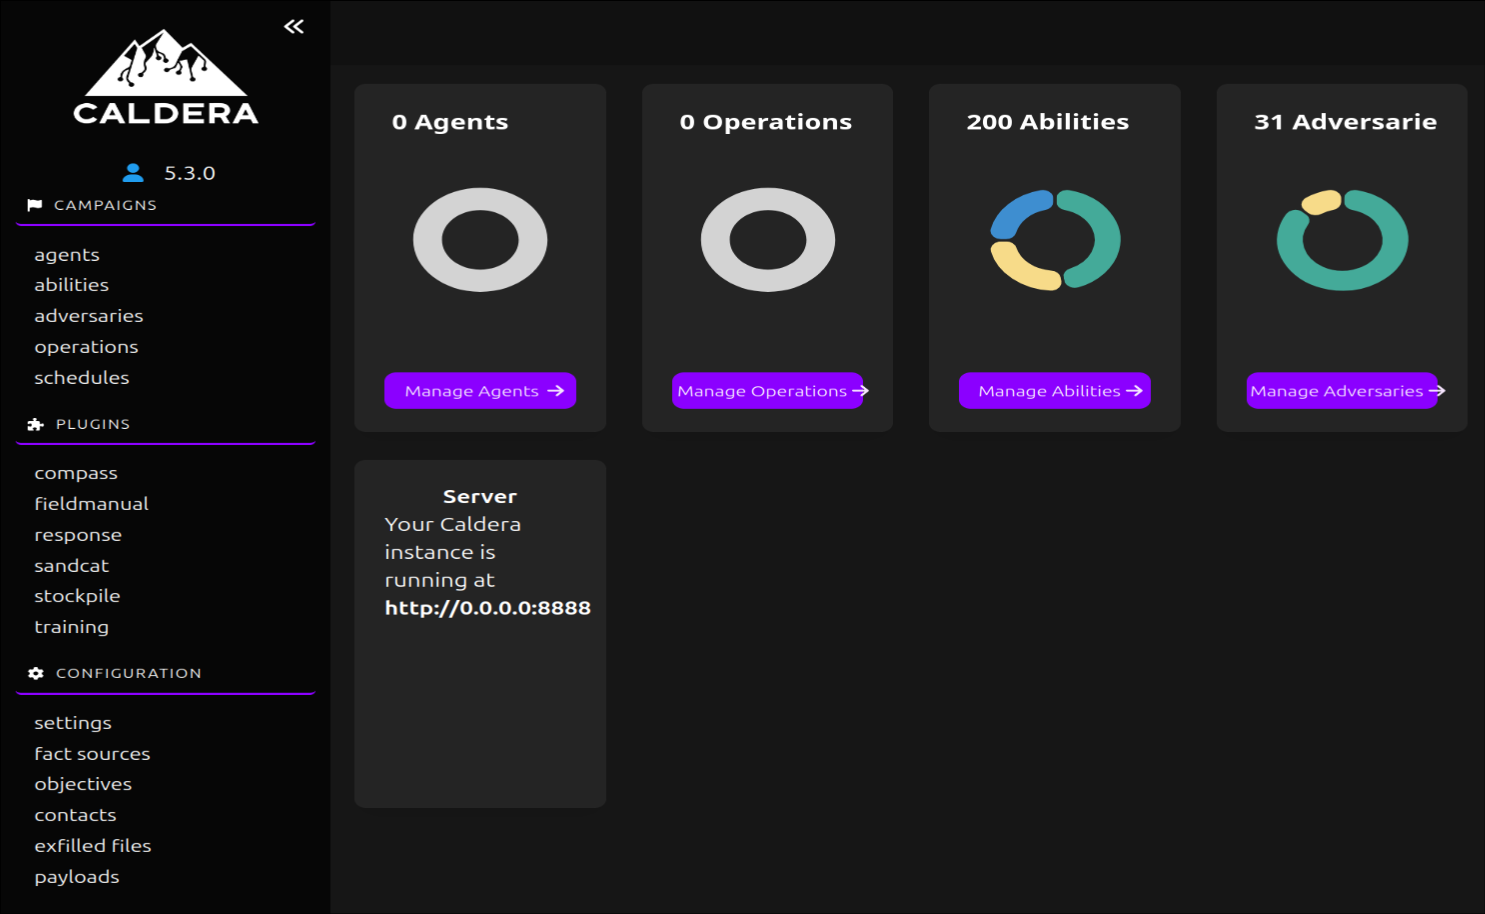
\includegraphics[width=\linewidth]{figures/Caldera_dashboard_blue.png}
    \caption{MITRE Caldera's Blue Dashboard}
    \label{fig:Caldera_dashboard_blue}
\end{figure}

\begin{itemize}
    \item \textbf{Knowledge and Operational Flow}\\
The platform's intelligence is driven by Facts, which are pieces of information (like IPs or usernames) about the network or host. These facts are collected by Parsers from the output of executed abilities and are crucial for the simulation's adaptive behavior, as they are used to substitute variables in subsequent commands, allowing the adversary to progress intelligently through an attack chain. The complete simulation is tracked through Operations, which record all actions. Caldera's functionality is sustained by clear technical prerequisites, requiring a Linux or macOS server with Python 3.8+ and NodeJS v16+, with GoLang 1.17+ recommended for dynamic agent compilation to aid in antivirus evasion. All server settings, C2 contacts, and API keys are managed through YAML configuration files.

\item \textbf{Core Capabilities and Plugins}\\
Caldera supports the full spectrum of cyber conflict through specialized capabilities and an extensive Plugin Architecture:
\begin{itemize}
    \item \textbf{Autonomous Red and Blue Engagements:} The framework facilitates fully Autonomous Red-Team Engagements to test defenses and Autonomous Incident-Response operations, where defensive profiles automatically execute counter-actions based on collected network facts.
    
    \item \textbf{Access and Movement:} The platform enables the simulation of initial intrusion stages, including Initial Access Attacks (Pre-ATT\&CK and Initial Access tactics) and Lateral Movement. Lateral movement, often seen in Windows environments, involves moving the agent binary to a new host and remotely executing it (via service creation or WMI) to establish a new C2 connection.
    
    \item \textbf{Exfiltration Methodology:} Data theft is a multi-step process governed by the Stockpile plugin. This involves first using the Advanced File Search and Stager ability to locate files and move them to a hidden staging directory. The staged files are then typically compressed, encrypted (often password-protected), and finally transferred to external destinations like Dropbox, GitHub, or AWS S3 that have been pre-configured in the Fact Source.
\end{itemize}

    \item \textbf{Key Plugin Functions:}
\begin{itemize}
    \item \textbf{Stockpile:} Serves as the core content repository for abilities and adversaries.
    \item \textbf{Sandcat:} Provides the flexible, modular agent that supports multiple C2 communication channels (HTTP(S), DNS Tunneling) and Peer-to-Peer Proxy capabilities via gocat extensions.
    \item \textbf{Response:} Offers content for autonomous defensive actions.
    \item \textbf{Debrief:} Provides campaign analytics, visualization, and detailed reporting.
    \item \textbf{Atomic:} Imports tests from the Red Canary Atomic repository for expanded emulation content.
\end{itemize}
\end{itemize}

Figure~\ref{fig:caldera_agents} shows the Agents management interface in Caldera, showing a deployed agent with a unique ID (paw), its host, assigned group (red), platform (linux), contact method (HTTP), and current status (alive, trusted). This interface allows operators to monitor and manage their implants across the network.

\begin{figure}
    \centering
    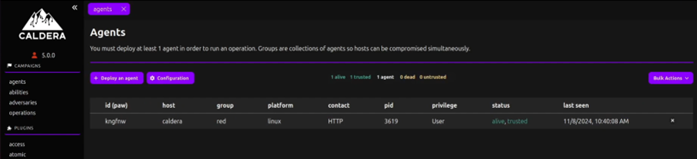
\includegraphics[width=1\linewidth]{figures/Figure22.png}
    \caption{MITRE Caldera’s Agents management}
    \label{fig:caldera_agents}
\end{figure}

The Abilities section, depicted in Figure~\ref{fig:caldera_abilities}, showcases the vast library of attack and defense techniques available within Caldera. Each entry represents a specific ATT\&CK tactic/technique, detailing its name (e.g., ``C2 Data Exfiltration'' or ``Compress Staged Directory''), the associated MITRE ATT\&CK ID (e.g., T1041 or T1560.001), and a brief description of its function. This interface allows users to search, filter by platform or plugin, and select the precise TTPs needed for their emulation scenarios.

\begin{figure}
    \centering
    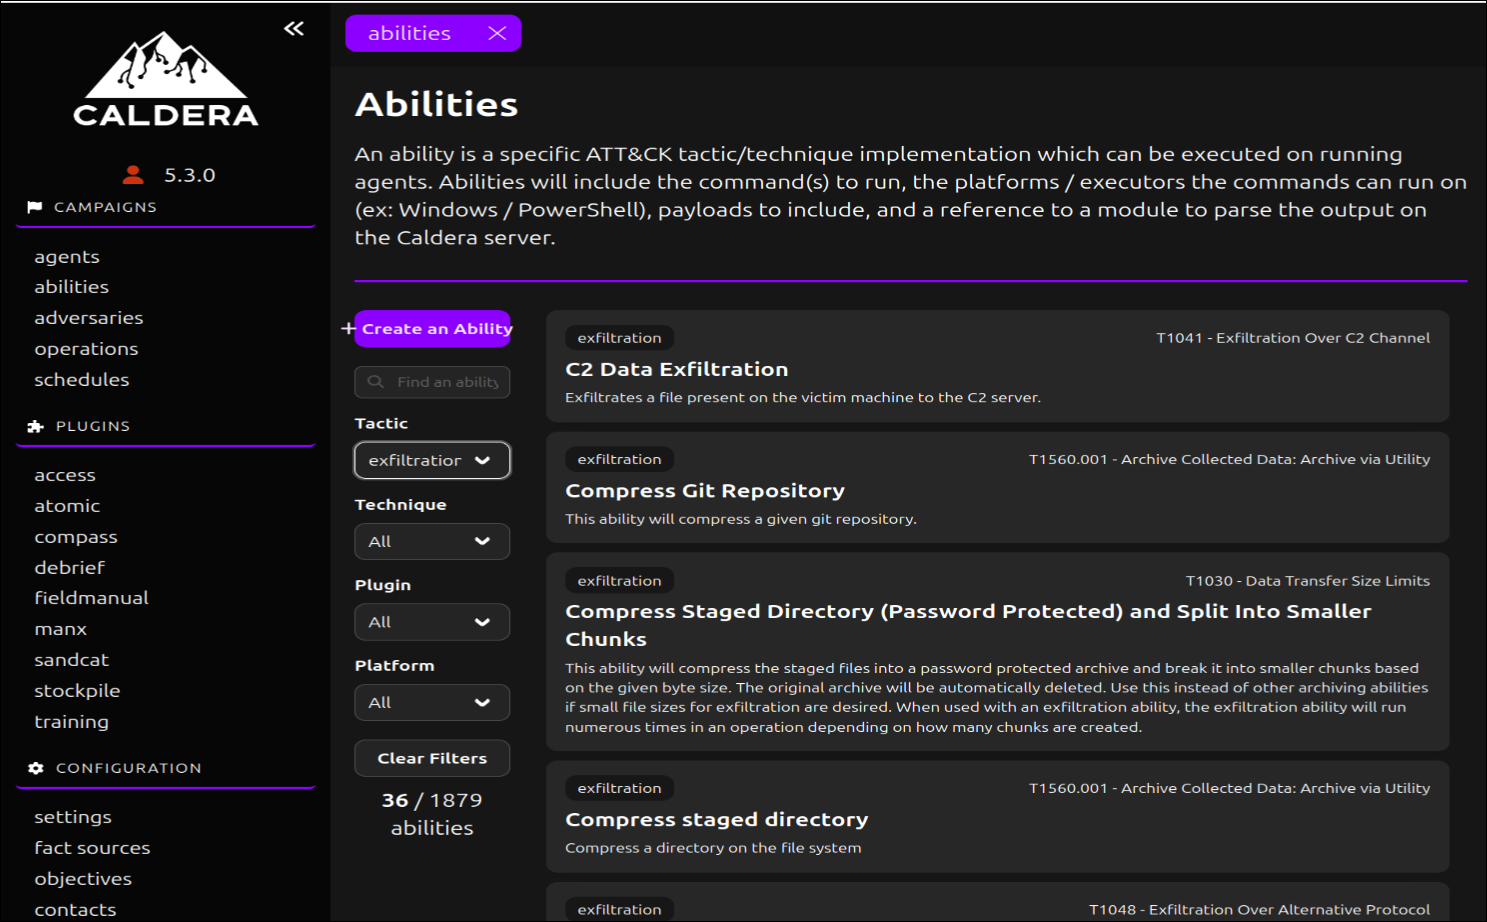
\includegraphics[width=1\linewidth]{figures/Caldera_Abilities.png}
    \caption{MITRE Caldera's Abilities interface}
    \label{fig:caldera_abilities}
\end{figure}

 \begin{itemize}
     \item \textbf{Analysis and Reporting}
 Upon completion of an operation, Caldera generates two essential, structured JSON reports for post-operation analysis, critical for forensic investigation and security monitoring evaluation:
    \begin{itemize}
    \item \textbf{Operation Report:} This is a comprehensive, nested summary that includes the full Adversary Profile, the selected Planner, the complete list of all Facts collected, and detailed, step-by-step execution records, along with their ATT\&CK mapping (Tactic and Technique ID). It is primarily used for deep forensic and research analysis.

    \item \textbf{Operation Event Logs:} This is a ``flattened'' list of execution events optimized for direct ingestion into SIEM tools. It focuses specifically on the successfully executed commands and includes agent/ability metadata, execution timestamps, and ATT\&CK mappings, allowing defenders to validate their security detection and logging capabilities against the simulated TTPs.
    \end{itemize}
\end{itemize}

%-----------------------------|    2.4 Infection Monkey    |------------------------------------|
\section{Infection Monkey}\label{sec:Infection}
Infection Monkey\cite{monkey_docs} is a comprehensive, open-source Breach and Attack Simulation (BAS) tool designed to continuously test an organization’s resilience against internal server infection and lateral movement. It safely simulates the behavior of a worm-like binary program, providing security teams with an empirical, attacker-centric view of their internal network to validate existing security controls and identify hidden security gaps.

\begin{figure}
    \centering
    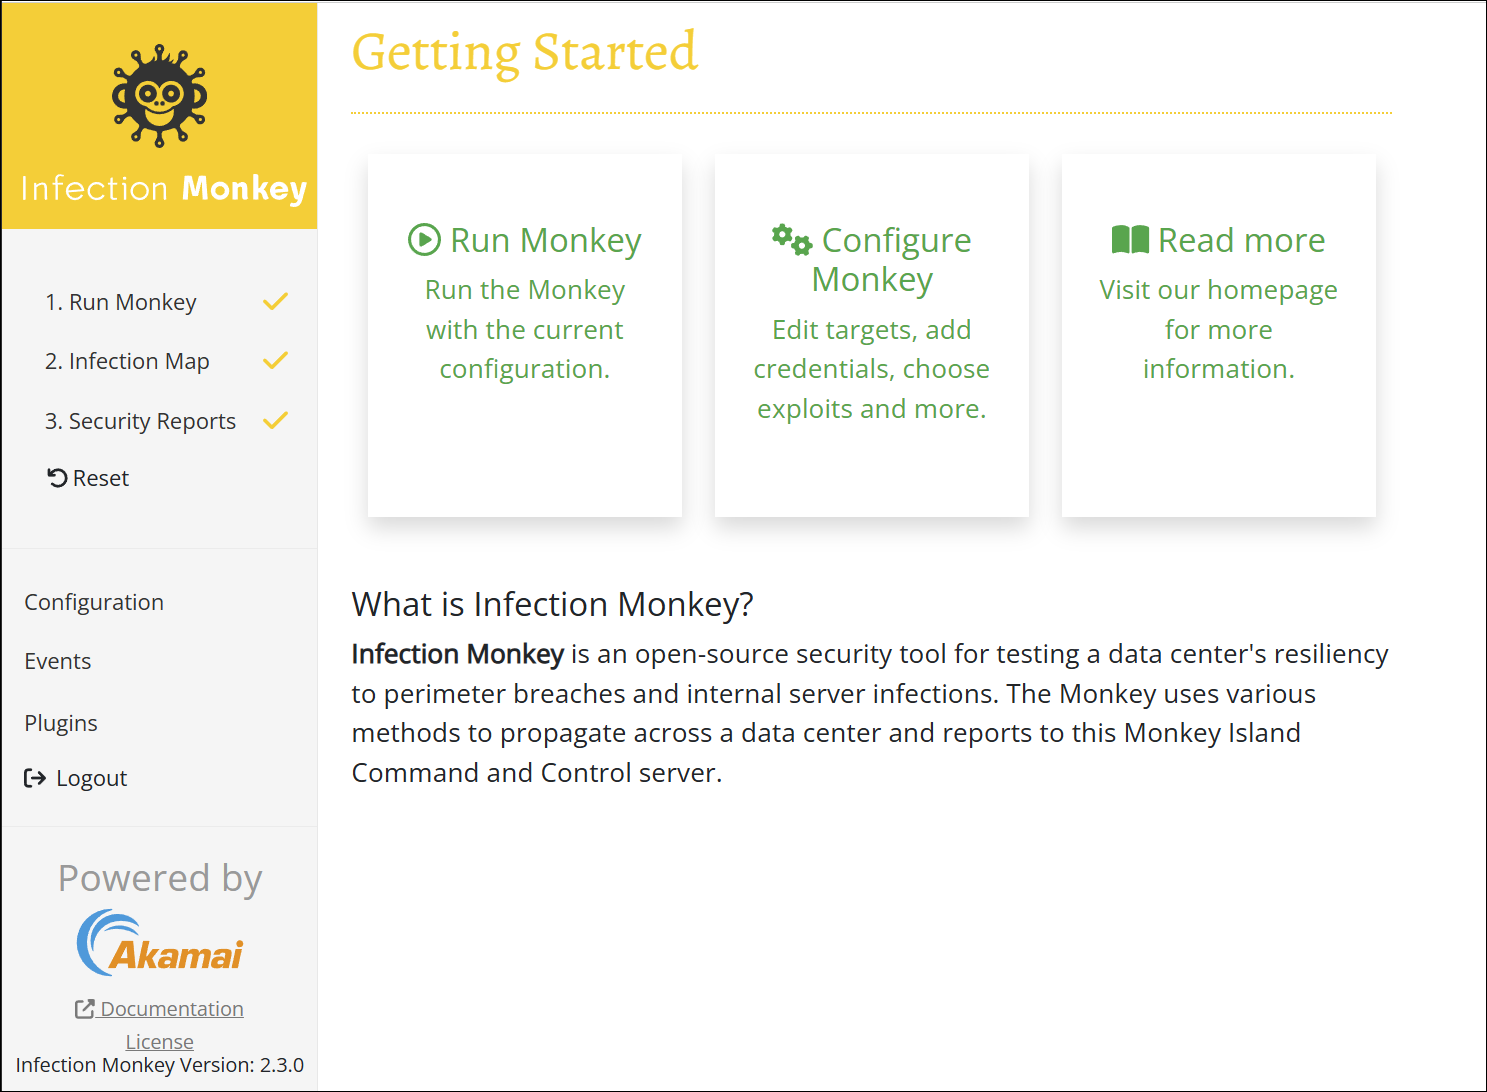
\includegraphics[width=1\linewidth]{figures/Getting Started.png}
    \caption{Infection Monkey's Island Dashboard }
    \label{fig:monkey_dashboard}
\end{figure}

Figure~\ref{fig:monkey_dashboard} displays the Monkey Island central dashboard. This interface provides direct access to essential workflows, allowing operators to configure attack parameters, launch simulations, and navigate to reporting modules via the sidebar.

\begin{itemize}
    \item \textbf{Core Architecture and Methodology}

The Infection Monkey platform is composed of two primary, communicating components:

\begin{itemize}
    \item \textbf{Monkey Agent (Monkey):} The core simulation tool. This is a safe, worm-like binary configured to autonomously scan the local network, attempt propagation to other machines using safe exploiters, and simulate various post-breach attack techniques without causing permanent damage.

    \item \textbf{Monkey Island Server (Island):} The centralized Command and Control (C\&C) web server. It handles the UI, manages the simulation configuration, aggregates all collected data, and presents the final reports and network visual maps.
\end{itemize}

The overall methodology centers on controlled network propagation. Agents spread based on pre-defined configuration parameters (which can include credentials, network segment rules, or specific attack scenarios), replicating an attacker's discovery and lateral movement techniques. The simulation uses only safe exploiters and is engineered to avoid permanent system modifications.
    \item \textbf{Simulation Capabilities and Scenarios}
Infection Monkey is highly versatile, offering core features and custom scenarios to fine-tune testing for specific defensive needs. The simulation workflow is enabled through an extensible plugin system and can be initiated either ``From Island'' (starting on the C\&C machine) or ``Manual'' (running the agent on a specific compromised host).
    \item \textbf{Key simulation capabilities and scenarios include:}
 \begin{itemize}
     \item \textbf{Ransomware Simulation:} Tests data manipulation defenses by simulating ransomware behavior. The agent encrypts files in a user-specified directory using a fully reversible bit-flip algorithm and replicates ransom note placement.
    \item \textbf{Network Breach:} Simulates lateral propagation starting from an already compromised internal host (e.g., a database server) to assess the blast radius of an initial breach.
    \item \textbf{Network Segmentation:}  Verifies the efficacy of isolation policies. Users define subnets that should be segregated, and the Monkey verifies isolation by attempting simple cross-segment ping tests. Isolation failures are detailed in the Security Report.
    \item \textbf{Credentials Leak:} Assesses the impact of stolen credentials. Users can input real credentials (usernames and passwords) or allow the Monkey to collect discovered SSH key pairs, which the agent then automatically reuses to facilitate lateral movement across the network.
 \end{itemize}

    \item \textbf{Platform and Deployment Support}

The platform is designed for broad accessibility, with all components running on x86-64 processors.

    \begin{itemize}
        \item The \textbf{Monkey Agent} offers a minimal footprint and supports a wide range of operating systems, including Linux (GLIBC $\ge$ 2.23) and Windows (Windows $\ge$ 2012).
    
        \item The \textbf{Monkey Island Server}, which serves as the central command and control, runs natively on modern Linux distributions (via AppImage) and Windows Server 2016/2019/Windows 10. Note that the server component requires significant resources, specifically a minimum of 4 CPU Cores and 6GB RAM for Windows Server environments.

        \item Deployment methods are flexible, including Windows Installer, Linux AppImage, Docker (Linux-only), and a dedicated AWS Marketplace AMI. The AMI deployment specifically requires inbound TCP traffic on port 5000.
\end{itemize}

Figure~\ref{fig:monkey_map} presents the Infection Map, which visualizes the attack topology. It depicts the central ``Monkey'' agent initiating network scans against discovered Windows targets, with orange directional lines indicating the flow of reconnaissance.

\begin{figure}
    \centering
    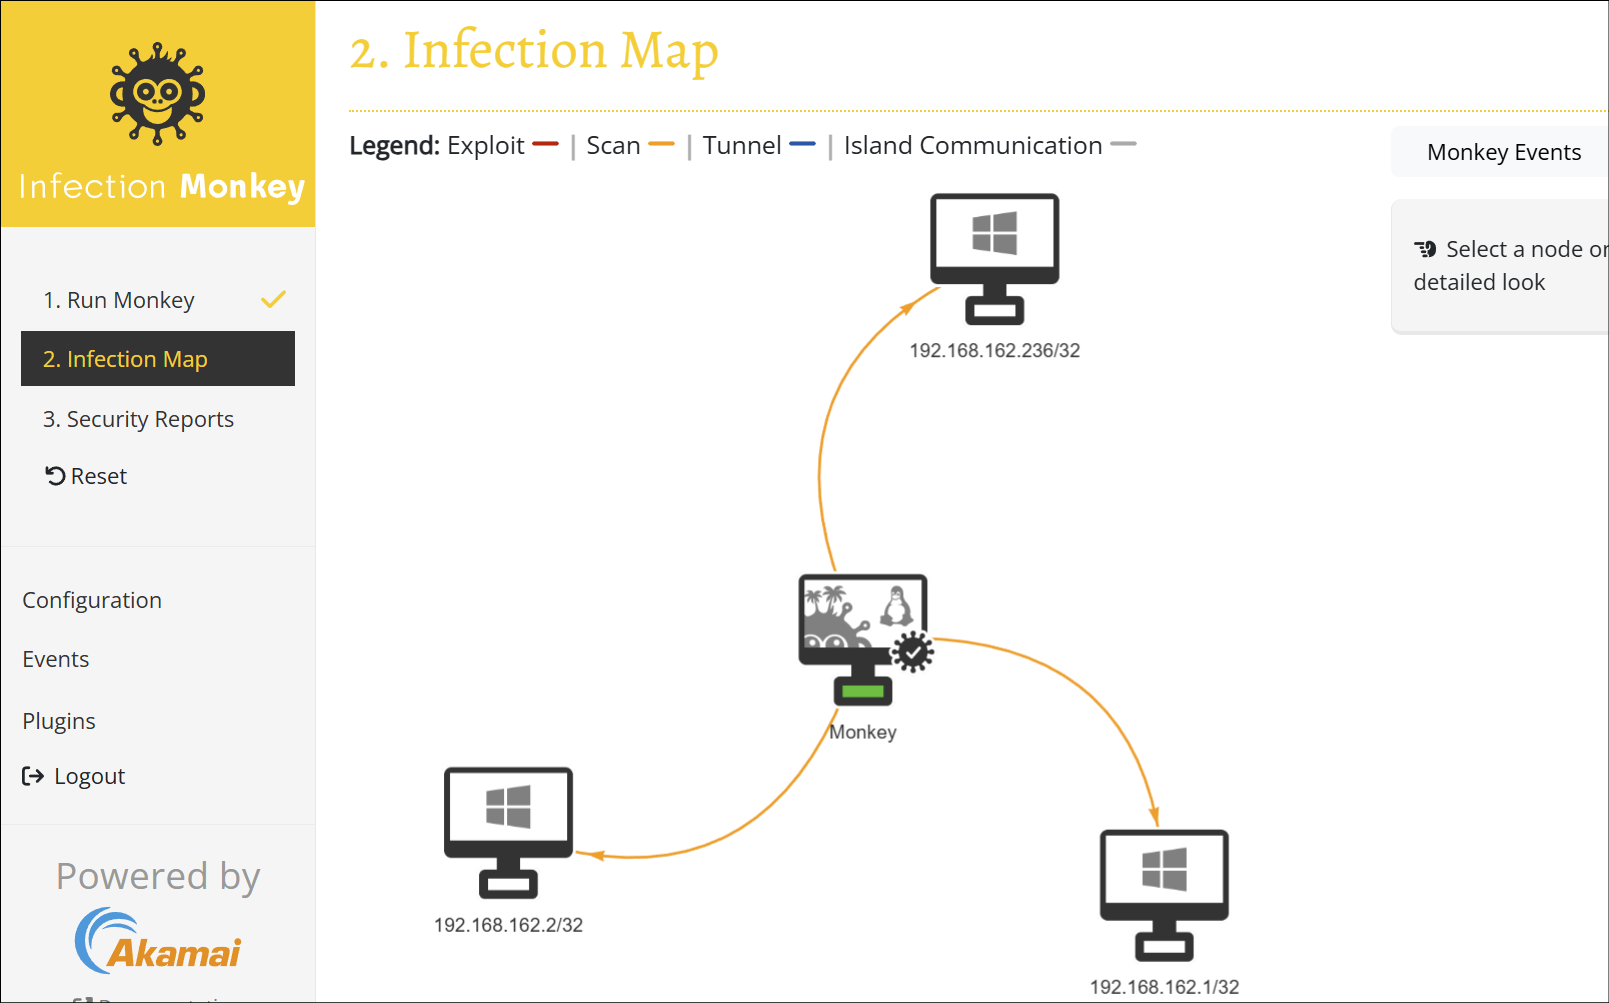
\includegraphics[width=1\linewidth]{figures/Infection Map.png}
    \caption{Infection Monkey's Network Propagation Map}
    \label{fig:monkey_map}
\end{figure}

    \item \textbf{Analysis and Reporting}

The results of the simulation are translated into actionable security improvements via detailed reports, primarily the Security Report. This comprehensive report provides mitigation steps and is organized into sections that detail:

         \begin{itemize}
             \item \textbf{Security Report:} The comprehensive primary report provides actionable mitigation steps and is split into sections that detail:
       
            \begin{enumerate}
                 \item High-Level Execution
                 \item Segmentation Issues
                 \item Machine-related Recommendations
                 \item The Network from the Monkey's Eyes (a summary of scanned, breached, and credential theft activities)
            \end{enumerate}

            \item \textbf{Ransomware Report}: A dedicated report that details the successful ransomware simulation in three sections:
            \begin{enumerate}
                 \item Breach (entry point)
                 \item Lateral Movement (propagation path)
                 \item Attack (list of specific files successfully encrypted)
            \end{enumerate}
        \end{itemize}
      \end{itemize}

\begin{figure}
    \centering
    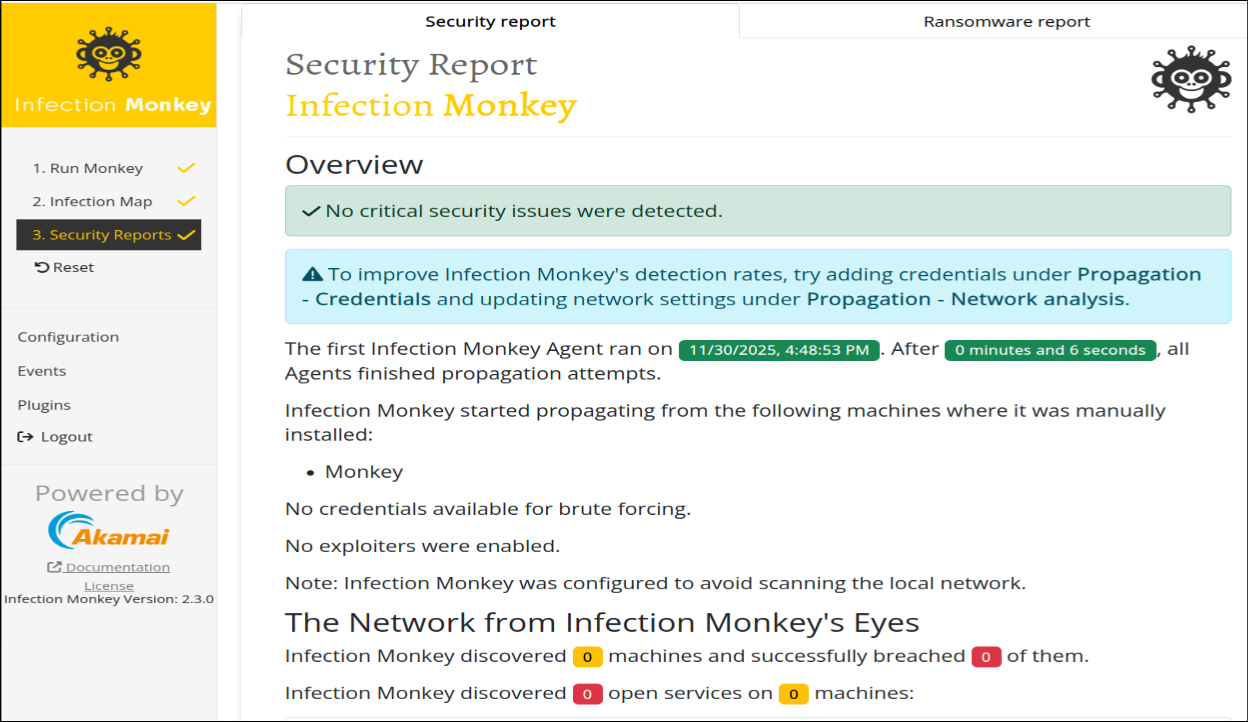
\includegraphics[width=1\linewidth]{figures/SecurityReport.png}
    \caption{Infection Monkey's Security Report}
    \label{fig:monkey_reports}
\end{figure}

Figure~\ref{fig:monkey_reports} shows an example of the Security Report in the Monkey Island UI. The overview highlights a critical security issue detected and details the attack's initiation, including the machine from which propagation started (island-linux-250), the usernames available for brute-forcing (e.g., Administrator, m0nk3y), and the sensitive credentials available for brute-forcing (e.g., LM hash, NT hash, Clear SSH private key, Clear Password). This section immediately demonstrates the quality of information an attacker could leverage and the starting point of the lateral movement within the network.

\begin{figure}[htbp]
    \centering
    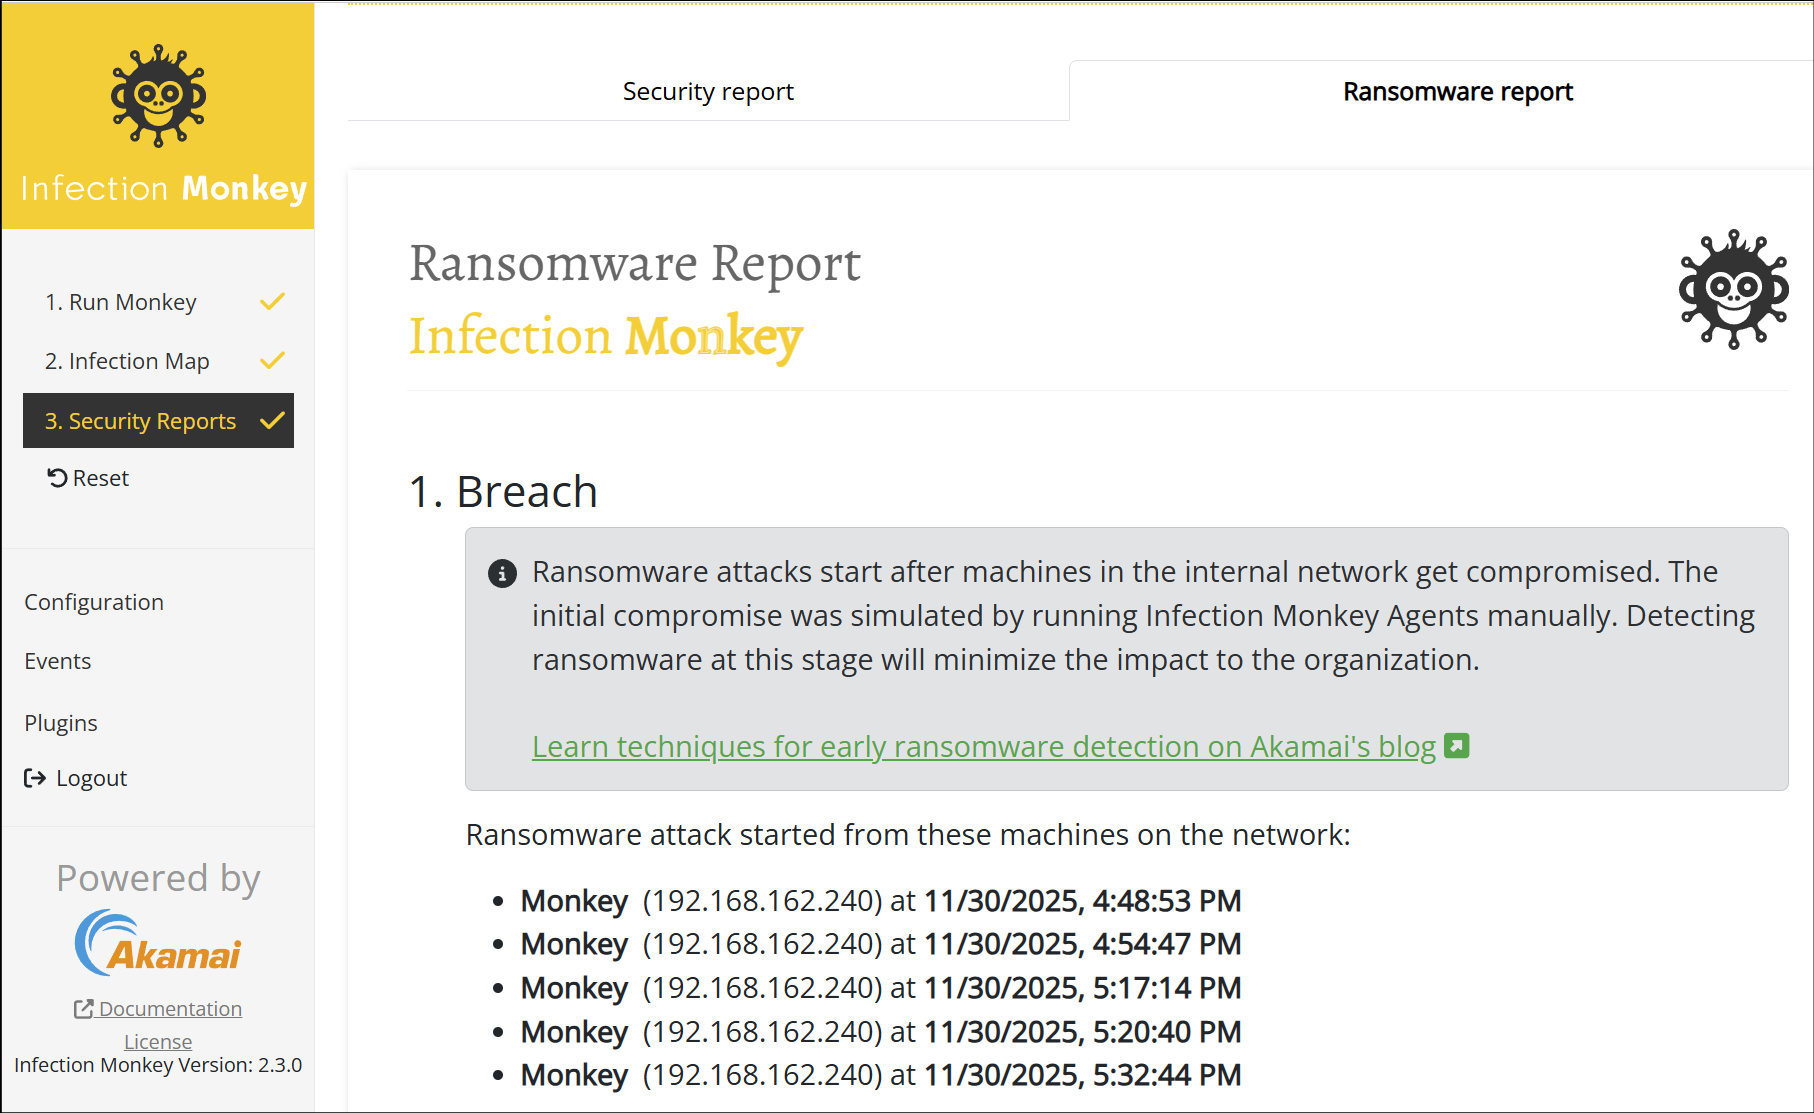
\includegraphics[width=1\linewidth]{figures/RansomwareReport.png}
    \caption{Infection Monkey's Ransomware Report}
    \label{fig:monkey_ransomware_report}
\end{figure}

Figure~\ref{fig:monkey_ransomware_report} displays the Ransomware Report interface. It details the initial ``Breach'' phase, logging the source machine (192.168.162.240) and specific execution timestamps. The report follows the attack chain, explicitly separating the initial entry point from subsequent lateral movement attempts.

%---------------------------|    2.5 Atomic Red Team   |---------------------------------------|
\section{Atomic Red Team}\label{sec:Atomic}
The Atomic Red Team\cite{atomic_docs} is a free and open-source library of scripted cyberattacks that serves as a fundamental resource for security teams seeking to systematically assess and validate their security controls. It functions as a community-driven, accessible alternative to proprietary Breach and Attack Simulation software. The project's primary objective is to operationalize adversary tradecraft by providing detailed procedures for defense validation.

\begin{figure}
    \centering
    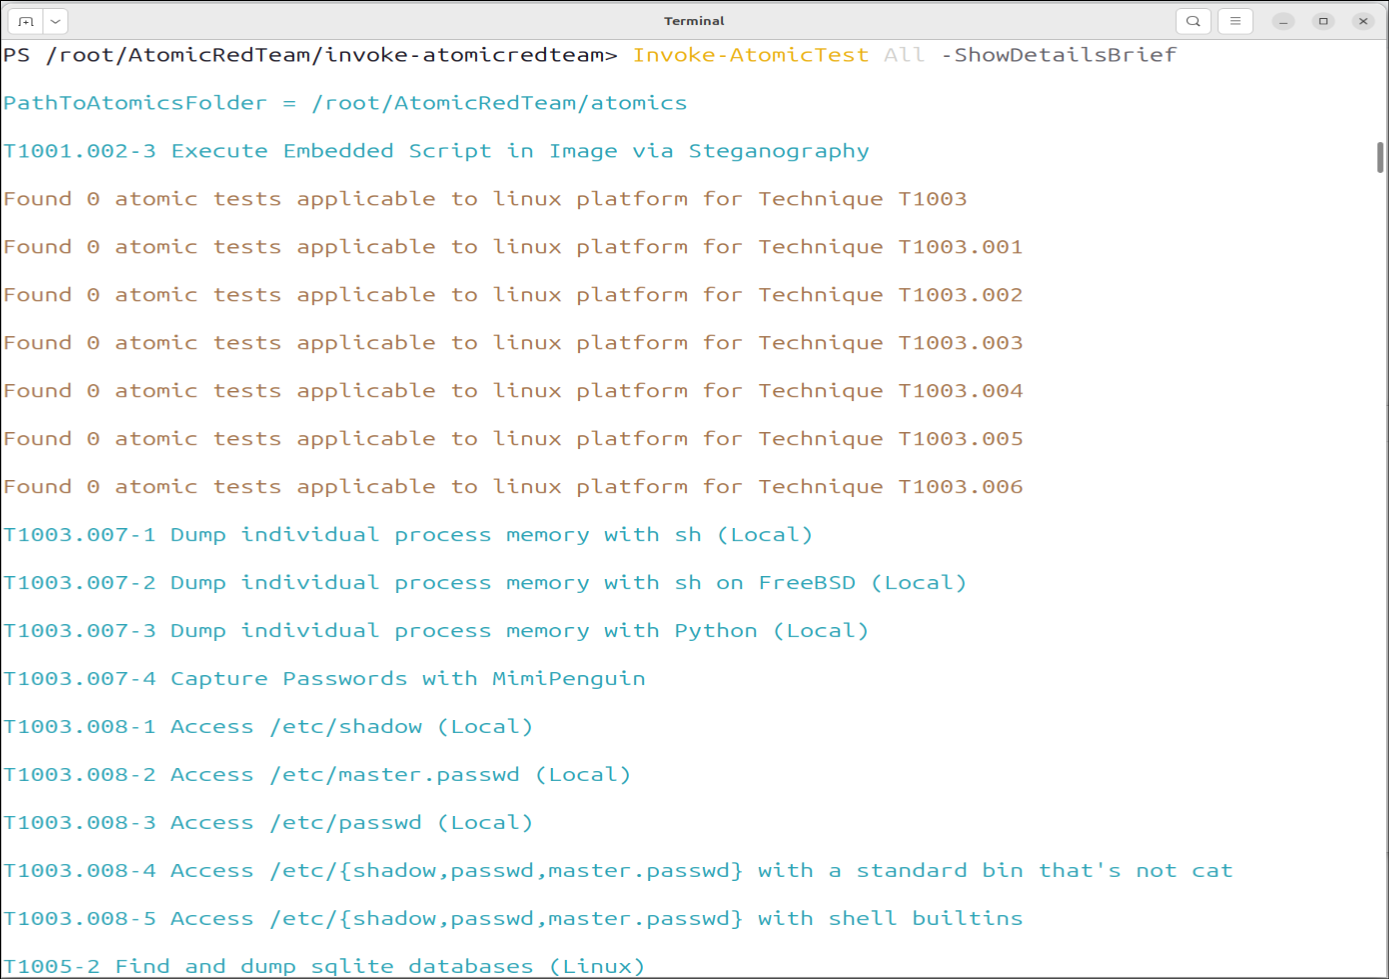
\includegraphics[width=1\linewidth]{figures/Canary_framework.png}
    \caption{Atomic Red Team's MITRE ATT\&CK lists}
    \label{fig:Canary_mitreid}
\end{figure}

Figure~\ref{fig:Canary_mitreid} displays the output of the \textit{Invoke-AtomicRedTeam} command. The framework filters and lists atomic tests applicable to the Linux platform, categorized by MITRE ATT\&CK technique IDs.

\begin{itemize}
    \item \textbf{Foundational Methodology}

The core methodology of the Atomic Red Team is its strict alignment with the MITRE ATT\&CK® matrix. The library fills a gap in the MITRE framework by translating abstract techniques into concrete, executable procedures, known as Atomic Tests.

    \item \textbf{Key characteristics of the tests include:}
        \begin{itemize}
            \item \textbf{Efficiency:} Designed to run quickly, often in five minutes or less.
             \item \textbf{Structure:} Each test is indexed by its MITRE ATT\&CK ID (T-number) and includes prerequisites, attack commands, optional cleanup commands, and input arguments for customization.
        \end{itemize}
    \item \textbf{Operational Frameworks and Tools}

The Atomic Red Team ecosystem provides several specialized, cross-platform tools to execute and validate the library's procedures.

\begin{itemize}
    \item \textbf{Invoke-AtomicRedTeam (Execution)}
    
Invoke-Atomic is the dedicated PowerShell execution framework used to manage and run the atomic tests, simplifying complex execution workflows.


\begin{itemize}
    \item \textbf{Capabilities:} It supports cross-platform execution (Windows, macOS, Linux) via PowerShell Core, enables remote execution through PowerShell remoting, and automates critical steps like checking and installing prerequisites (Get Prereq Commands), substituting input arguments, and running cleanup commands.

    \item \textbf{Atomic Runner:} A component of the framework designed for enterprise use, facilitating the orchestration of scheduled tests across multiple machines and ensuring proper logging via unique GUIDs and host names for detection correlation.
\end{itemize}

\item \textbf{Specialized Validation Tools}
        \begin{itemize}
            \item \textbf{AtomicTestHarnesses:} A library (utilizing PowerShell and Python) crucial for validating the telemetry generated during execution. It is designed to stress test detection systems by running many variations of a single technique to evaluate the depth and fragility of security coverage.
            \item \textbf{Chain Reactor:} An open-source framework dedicated to composing executables that simulate adversary behaviors specifically on Linux endpoints. It uses easily configurable JSON input files.
        \end{itemize}
    \end{itemize}
    \item \textbf{Test Design and Contribution Standards}

The community-driven nature of Atomic Red Team necessitates strict guidelines for test development to ensure consistency and utility.

\begin{itemize}
    \item \textbf{Cleanup and Dependencies:} Cleanup commands must be designed to be repeatable without generating errors. External dependencies should not be committed directly but must be downloaded from their original sources using the prereq commands YAML key, often via permanent GitHub links.

    \item \textbf{Portability:} New tests must be as portable as possible, relying on environment variables instead of hard-coded paths, and favoring \texttt{sh} over \texttt{bash} for Linux.

    \item \textbf{Documentation:} Tests must be accompanied by clear descriptions, the expected output, and links to external resources that detail the attack.
\end{itemize}

    \item \textbf{Best Practices and Security Responsibility}

The framework's core value is its capacity to move an organization past security based on ``hope''.

\begin{itemize}
    \item \textbf{Testing Philosophy:} Best practice dictates testing should occur in two phases: first, with blocking controls OFF to ensure comprehensive detection telemetry is collected, and second, with blocking controls ON to evaluate prevention efficacy. The guiding principle cited is: ``Prevention is ideal, but detection is a must''.

    \item \textbf{Safety and Responsibility:} Users must always obtain permission before testing and execute all procedures in a dedicated non-production or lab environment, as tests may leave the system in an undesirable state.
    \end{itemize}
\end{itemize}
\begin{figure}[htbp]
    \centering
    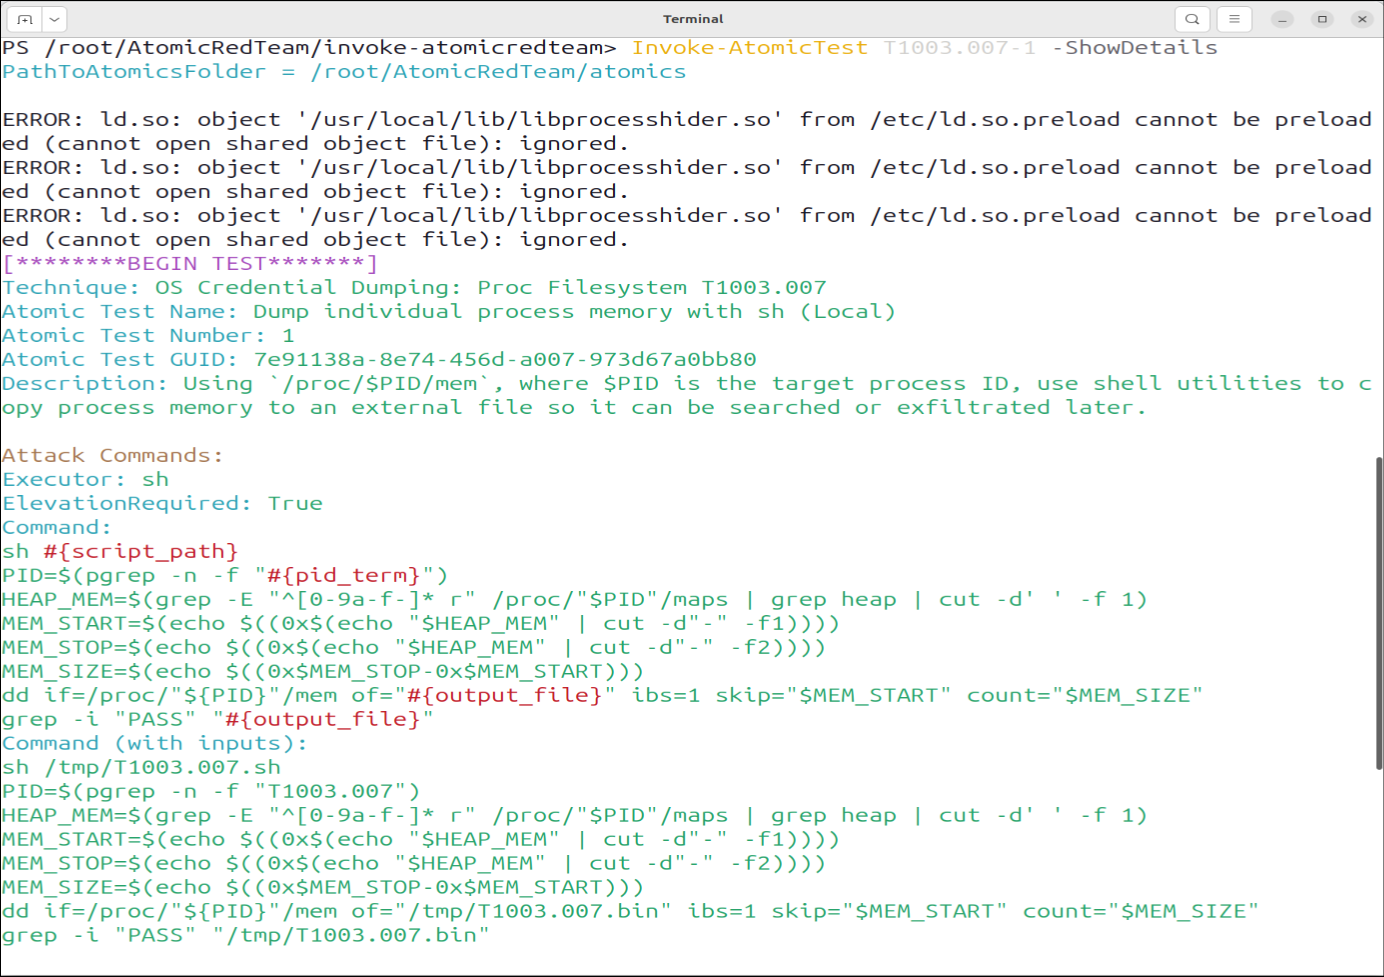
\includegraphics[width=1\linewidth]{figures/Canary_EX-Attack.png}
    \caption{Atomic Red Team's execution logic example}
    \label{fig:example_attack}
\end{figure}

Figure~\ref{fig:example_attack} shows an example of the detailed configuration for Atomic Test T1003.007-1, which simulates OS Credential Dumping via the Proc Filesystem. The output reveals the specific shell commands utilized to perform the attack, demonstrating how the \texttt{dd} utility is used to extract the heap memory of a target process from \texttt{/proc/\$PID/mem} for credential analysis.

%---------------------------|    2.6 Related Work   |--------------------------------------|
\section{Related Work}
The shift from manual penetration testing to automated security validation is a major trend in cybersecurity. However, few studies directly compare open-source Breach and Attack Simulation (BAS) tools. Most existing research focuses either on qualitative feature comparisons or theoretical models. 

\subsection{Red Team Redemption: A Structured Comparison of Open-Source Tools for Adversary Emulation}
Landauer et al.\cite{landauer2024} provide a foundational baseline in their work, "Red Team Redemption," which conducted a comprehensive survey and ranking of 9 adversary emulation tools: ATTPwn, Atomic Red Team, APTSimulator, MITRE Caldera, DumpsterFire, Infection Monkey, Invoke Adversary, Metaspoit and Purplesharp. Their study utilized a mixed-method approach comprising three interconnected components that all relied on a single master list of features:
\begin{itemize}
    \item \textbf{Questionnaire Assessment:} The establishment of a theoretical framework evaluating 80 specific criteria across 5 core categories: Installation \& Configuration, Community \& Support, Documentation, Usability, and Features \& Capabilities.
    \item \textbf{Offline Tool Assessment:} A hands-on technical evaluation to verify basic functional requirements, utilizing offline checklists that directly mapped to the 80 criteria established in the questionnaire phase.
    \item \textbf{User Requirement Survey:} A survey asking cybersecurity domain experts to assign importance weights to these exact same 80 criteria in order to calculate an overall tool ranking.
\end{itemize}

While Landauer’s 80-question framework provides a foundational taxonomy, this study operationalizes these criteria through a high-fidelity laboratory environment. By narrowing the scope to Installation \& Configuration and Features \& Capabilities, the research transitions from qualitative assessment to direct technical verification. This approach focuses exclusively on reproducible telemetry—such as exact deployment sequences, resource overhead, and execution stability—while intentionally excluding subjective, survey-based categories like Documentation and Usability. This ensures the evaluation is grounded in the empirical reality of tool deployment rather than aesthetic or manual-based preferences.

\subsection{A Unified Modeling Framework for Automated Penetration Testing}
Wang et al. \cite{wang2025} address the theoretical fragmentation in automated penetration testing (AutoPT) by proposing a standardized modeling framework. Analyzing and categorizing 65 studies, they introduced the Multi-Dimensional Classification System (MDCPM) and a practical simulation engine to support AI agent training. Their work comprises three core components:
\begin{itemize}
    \item \textbf{MDCPM Classification:} A theoretical system categorizing literature into four dimensions: Literature Objectives, Network Complexity, Dependency of Technical and Tactical Operations, and Scenario Feedback.
    \item \textbf{AutoPT-Sim Framework:} A unified modeling framework designed to simulate dynamic network environments, attackers, and defenders.
    \item \textbf{Public Dataset and Generator:} The release of a standard network environment dataset and a "Network Generator" tool for fair algorithm comparison.
\end{itemize}

While Wang et al. provide a robust theoretical foundation, their framework relies on abstract models rather than empirical software execution. This research bridges that gap by operationalizing their MDCPM classification within a controlled laboratory environment. Specifically, their requirement for dynamic scenario feedback is translated into our Threat Intelligence Alignment evaluation, while the need for coordinated technical operations is verified through Framework Extensibility testing. Furthermore, while Wang theoretically validates MITRE Caldera, they identify a scarcity of dynamically updated scenarios; we address this by empirically benchmarking tool update mechanisms and repository health. This transitions Wang’s theoretical concepts into reproducible laboratory parameters derived from the actual installation and execution of each BAS tool. 

\subsection{Cyber Attack Modeling and Simulation for Network Security Analysis}
Addressing the limitations of physical testbeds, Kuhl et al. \cite{kuhl2007} developed a discrete-event simulation framework to model computer networks and generate synthetic security data. Their work focused on creating a flexible environment for testing situational awareness tools through three core mechanisms:
\begin{itemize}
    \item \textbf{Network Abstraction:} They modeled infrastructure using logical constructs to represent network topology efficiently, specifically designed to avoid the computational overhead of packet-level simulation.
    \item \textbf{Multi-Stage Attack Generation:} Leveraging a graph-based guidance template, they implemented an attack model spanning ten distinct stages (from Reconnaissance to Goal/Pilfering), pre-dating but mirroring the structure of the MITRE ATT\&CK framework.
    \item \textbf{Synthetic Data Production:} The simulation generated comprehensive output datasets, providing "ground truth" logs of attacker actions mixed with background noise for defensive validation.
\end{itemize}

While Kuhl et al. prioritized scalability through abstraction, their approach inherently masks the physical impact of attack emulation on host systems. This study builds upon Kuhl’s concepts but shifts from a simulated environment to a high-fidelity physical laboratory. Specifically, where Kuhl sought to avoid 'computational overhead' through modeling, we treat system resource overhead as a primary performance indicator to quantify the actual hardware costs of BAS deployment. Furthermore, Kuhl’s 10-stage attack model underscores the necessity of evaluating Scenario Coverage for threat relevance in a live environment. Finally, whereas Kuhl produced 'synthetic ground truth logs,' this research evaluates the empirical execution reliability of actual malware payloads, ensuring that multi-stage attacks can execute without destabilizing the host during real-world installation.

\subsection{Implementation of Security Controls for the Treatment of Malware using Breach and Attack Simulation}

Focusing on the mitigation of ransomware and zero-day threats, Roque et al. \cite{roque2024} proposed a security architecture that integrates Breach and Attack Simulation (BAS) technology with the National Institute of Standards and Technology (NIST) framework. Their research aimed to optimize security controls through a continuous validation process:
\begin{itemize}
    \item \textbf{Architectural Design:} They implemented a layered defense strategy mapped to the NIST phases, utilizing Snort for IPS/IDS rules and Microsoft Defender for EDR.
    \item \textbf{Simulated Attack Execution:} Using the Picus Security platform as the BAS tool, they conducted randomized simulations of specific threats, such as the BlackByte Ransomware campaign.
    \item \textbf{Iterative Optimization:} Based on simulation findings, they refined security policies to address identified gaps, increasing their threat detection rate from an initial 47\% to 95\%.
\end{itemize}

While Roque et al. demonstrate that a BAS platform's value lies in its actionable output, their methodology is tethered to a premium commercial ecosystem. Their reported 95\% detection rate was achieved through high-fidelity remediation data from Picus to calibrate Snort and EDR signatures—a luxury often absent in non-commercial environments. This study addresses the resulting accessibility gap by investigating whether open-source alternatives can achieve operational parity. We operationalize Roque’s findings into our Quality of Reports evaluation, moving beyond simple binary logs to measure the presence of remediation intelligence, such as pre-configured signatures or automated fix scripts. By executing these tools in a physical laboratory, this research empirically tests if open-source frameworks can provide the remediation depth necessary to meet professional operational standards.


\subsection{The Research Gap}

Despite these foundational contributions, there is a critical lack of empirical evaluation of open-source BAS tools in real operational environments. While previous studies established theoretical needs or utilized commercial platforms, the following gaps remain, directly informing the Comparison Matrix of this study:
\begin{itemize}
    \item \textbf{Lack of Reliability Testing:} Studies like Landauer et al. \cite{landauer2024} used qualitative "functional checklists" to verify if features existed. They did not perform stress testing to measure actual execution reliability (i.e., whether the tools crash or fail when executed repeatedly in a live environment), which this study addresses through accurate Execution Reliability scoring.
    \item \textbf{No Resource Usage Data:} Theoretical frameworks (Wang et al. \cite{wang2025}), simulation models (Kuhl et al. \cite{kuhl2007}), and practical implementations (Roque et al. \cite{roque2024}) entirely omit system overhead measurements. Consequently, there is no existing empirical data on the actual computational cost (CPU and memory usage) of running these BAS servers. This study introduces a novel Operational Performance evaluation  to measure this critical factor for resource-constrained enterprises.
    \item \textbf{Actionable Output vs. Open-Source Reality:} While Roque et al. \cite{roque2024} validated that actionable reporting is mandatory for improving defenses, they relied on a premium commercial tool (Picus). There is currently no systematic comparison of whether free, open-source alternatives can generate the same caliber of actionable remediation data. This study directly tests this capability through the Quality of Reports assessment.
\end{itemize}

\begin{table}
    \caption{Literature Review Gap Analysis}
    \label{tab:gap_analysis}
    \centering
    \renewcommand{\arraystretch}{1.8} % Increases row height for better breathing room
    \begin{tabular}{>{\raggedright\arraybackslash}m{0.25\linewidth} >{\raggedright\arraybackslash}m{0.30\linewidth} >{\raggedright\arraybackslash}m{0.38\linewidth}}
        \toprule
        \textbf{Research} & \textbf{Limitation (The Gap)} & \textbf{How This Study Addresses It} \\ 
        \midrule
        
        Landauer et al. [16] & 
        Qualitative only; lacks real performance stress-testing. & 
        Replaces surveys with \textbf{empirical telemetry} for reliability and deployment. \\ \cmidrule(lr){1-3}
        
        Wang et al. [17] & 
        Purely theoretical; relied on abstract models. & 
        \textbf{Operationalizes} requirements into measurable laboratory tests. \\ \cmidrule(lr){1-3}
        
        Kuhl et al. [18] & 
        Used synthetic logs and abstracted overhead. & 
        Captures \textbf{physical laboratory measurements} of system overhead. \\ \cmidrule(lr){1-3}
        
        Roque et al. [19] & 
        Limited exclusively to a single premium platform (Picus). & 
        Evaluates \textbf{functional equivalence} in open-source remediation data. \\ 
        \bottomrule
    \end{tabular}
\end{table}

Table~\ref{tab:gap_analysis} summarizes the specific limitations of these foundational studies and illustrates exactly how this research addresses those outstanding gaps through targeted empirical metrics.

This study directly addresses these deficiencies by transitioning from abstract simulations and proprietary ecosystems to a reproducible, high-fidelity laboratory environment. By executing open-source BAS tools on physical hardware, this research generates original empirical telemetry regarding operational performance, execution stability, and deployment complexity—data points currently absent from the existing body of knowledge.